
%%%%%%%%%%%%%%%%%%%%%%%%%%%%%%%%%%%%%%%%%%%%%%%%%%%%%%%%
\documentclass[12pt,a4paper]{article}% 文档格式
\usepackage{ctex,hyperref}% 输出汉字
\usepackage{times}% 英文使用Times New Roman
%%%%%%%%%%%%%%%%%%%%%%%%%%%%%%%%%%%%%%%%%%%%%%%%%%%%%%%%
\title{\fontsize{18pt}{27pt}\selectfont% 小四字号,1.5倍行距
	{\heiti% 黑体 
		相对论复习}}% 题目
%%%%%%%%%%%%%%%%%%%%%%%%%%%%%%%%%%%%%%%%%%%%%%%%%%%%%%%%
\author{\fontsize{12pt}{18pt}\selectfont% 小四字号,1.5倍行距
	{\fangsong% 仿宋
		香饽饽}\\% 标题栏脚注
	\fontsize{10.5pt}{15.75pt}\selectfont% 五号字号,1.5倍行距
	{\fangsong% 仿宋
		(复旦大专物理学系
		)}}% 作者单位,“~”表示空格
%%%%%%%%%%%%%%%%%%%%%%%%%%%%%%%%%%%%%%%%%%%%%%%%%%%%%%%%
\date{}% 日期(这里避免生成日期)
%%%%%%%%%%%%%%%%%%%%%%%%%%%%%%%%%%%%%%%%%%%%%%%%%%%%%%%%
\usepackage{amsmath,amsfonts,amssymb}% 为公式输入创造条件的宏包
%%%%%%%%%%%%%%%%%%%%%%%%%%%%%%%%%%%%%%%%%%%%%%%%%%%%%%%%
\usepackage{graphicx}% 图片插入宏包
\usepackage{subfigure}% 并排子图
\usepackage{float}% 浮动环境,用于调整图片位置
\usepackage[export]{adjustbox}% 防止过宽的图片
\usepackage{pdfpages}
\usepackage{tikz}
%%%%%%%%%%%%%%%%%%%%%%%%%%%%%%%%%%%%%%%%%%%%%%%%%%%%%%%%
\usepackage{bibentry}
\usepackage{natbib}% 以上2个为参考文献宏包
%%%%%%%%%%%%%%%%%%%%%%%%%%%%%%%%%%%%%%%%%%%%%%%%%%%%%%%%
\usepackage{abstract}% 两栏文档,一栏摘要及关键字宏包
\renewcommand{\abstracttextfont}{\fangsong}% 摘要内容字体为仿宋
\renewcommand{\abstractname}{\textbf{摘\quad 要}}% 更改摘要二字的样式
%%%%%%%%%%%%%%%%%%%%%%%%%%%%%%%%%%%%%%%%%%%%%%%%%%%%%%%%
\usepackage{xcolor}% 字体颜色宏包
\newcommand{\red}[1]{\textcolor[rgb]{1.00,0.00,0.00}{#1}}
\newcommand{\blue}[1]{\textcolor[rgb]{0.00,0.00,1.00}{#1}}
\newcommand{\green}[1]{\textcolor[rgb]{0.00,1.00,0.00}{#1}}
\newcommand{\darkblue}[1]
{\textcolor[rgb]{0.00,0.00,0.50}{#1}}
\newcommand{\darkgreen}[1]
{\textcolor[rgb]{0.00,0.37,0.00}{#1}}
\newcommand{\darkred}[1]{\textcolor[rgb]{0.60,0.00,0.00}{#1}}
\newcommand{\brown}[1]{\textcolor[rgb]{0.50,0.30,0.00}{#1}}
\newcommand{\purple}[1]{\textcolor[rgb]{0.50,0.00,0.50}{#1}}% 为使用方便而编辑的新指令
\renewcommand{\d}{\mathrm{d}}
%%%%%%%%%%%%%%%%%%%%%%%%%%%%%%%%%%%%%%%%%%%%%%%%%%%%%%%%
\usepackage{url}% 超链接
\usepackage{bm}% 加粗部分公式
\usepackage{multirow}
\usepackage{booktabs}
\usepackage{epstopdf}
\usepackage{epsfig}
\usepackage{longtable}% 长表格
\usepackage{supertabular}% 跨页表格
\usepackage{algorithm}
\usepackage{algorithmic}
\usepackage{changepage}% 换页
%%%%%%%%%%%%%%%%%%%%%%%%%%%%%%%%%%%%%%%%%%%%%%%%%%%%%%%%
\usepackage{enumerate}% 短编号
\usepackage{caption}% 设置标题
\captionsetup[figure]{name=\fontsize{10pt}{15pt}\selectfont Figure}% 设置图片编号头
\captionsetup[table]{name=\fontsize{10pt}{15pt}\selectfont Table}% 设置表格编号头
%%%%%%%%%%%%%%%%%%%%%%%%%%%%%%%%%%%%%%%%%%%%%%%%%%%%%%%%
%\usepackage{indentfirst}% 中文首行缩进
\usepackage[left=2.50cm,right=2.50cm,top=2.80cm,bottom=2.50cm]{geometry}% 页边距设置
\renewcommand{\baselinestretch}{1.5}% 定义行间距(1.5)
%%%%%%%%%%%%%%%%%%%%%%%%%%%%%%%%%%%%%%%%%%%%%%%%%%%%%%%%
\usepackage{fancyhdr} %设置全文页眉、页脚的格式
\pagestyle{fancy}
\hypersetup{colorlinks=true,linkcolor=black}% 去除引用红框,改变颜色
%%%%%%%%%%%%%%%%%%%%%%%%%%%%%%%%%%%%%%%%%%%%%%%%%%%%%%%%
\usepackage{caption}%标题取消自动figure
\usepackage{multicol}
\usepackage{cuted}
%%%%%%%%%%%%%%%%%%%%%%%%%%%%%%%%%%%%%%%%%%%%%%%%%%%%%%%%
%\usepackage{CJKutf8}
%%%%%%%%%%%%%%%%%%%%%%%%%%%%%%%%%%%%%%%%%%%%%%%%%%%%%%%
\newcommand{\nonumbersection}[1]{
	\section*{#1}
	\addcontentsline{toc}{section}{#1}
}
\newcommand{\nonumbersubsection}[1]{
	\subsection*{#1}
	\addcontentsline{toc}{subsection}{#1}
}
\newcommand{\csection}[1]{
	\subsection*{\centering{\huge{\textbf{#1}}}}
	\addcontentsline{toc}{subsection}{\texorpdfstring{\protect\numberline{}#1}{#1}}
}

\begin{document}% 以下为正文内容
	\maketitle% 产生标题,没有它无法显示标题
	%%%%%%%%%%%%%%%%%%%%%%%%%%%%%%%%%%%%%%%%%%%%%%%%%%%%%%%%
	\lhead{}% 页眉左边设为空
	\chead{}% 页眉中间设为空
	\rhead{}% 页眉右边设为空
	\lfoot{}% 页脚左边设为空
	\cfoot{\thepage}% 页脚中间显示页码
	\rfoot{}% 页脚右边设为空
	%%%%%%%%%%%%%%%%%%%%%%%%%%%%%%%%%%%%%%%%%%%%%%%%%%%%%%%%
	\begin{abstract}
	\fangsong 期末复习相对论,保佑我力学不挂科。相对论有一堆公式,而且丑的一批,还很难理解,要经常复习。
	\end{abstract}
	
	\begin{adjustwidth}{1.06cm}{1.06cm}
	\fontsize{10.5pt}{15.75pt}\selectfont{\heiti{关键词:}\fangsong{期末,力学}}\\
	\end{adjustwidth}
	
	%\begin{center}% 居中处理
	%	{\textbf{Abstract}}% 英文摘要
	%\end{center}
	%\begin{adjustwidth}{1.06cm}{1.06cm}% 英文摘要内容
	%	\hspace{1.5em}In order to improve my computer and English skills, please allow me to complete this physics homework in English context with \LaTeX, so as to improve my professional level. Sorry for the inconvenience!
	%\end{adjustwidth}
	
	\newpage% 从新的一页继续
	
	\renewcommand{\contentsname}{目录}
	\tableofcontents
	\newpage
	
	\csection{Lorentz 变换}
	 \noindent 我们都学过狭义相对论, Lorentz 变换可以写成矩阵的形式:
$$
\left( \begin{array}{c}
	ct'\\
	x'\\
\end{array} \right) =\widehat{\mathbf{Lor}}\left( \begin{array}{c}
	ct\\
	x\\
\end{array} \right) 
$$
	其中, $\mathbf{\widehat{Lor}}$ \text{表示 Lorentz 变换矩阵}:
	$$
	\widehat{\mathbf{Lor}}=\left( \begin{matrix}
		\gamma&		-\beta \gamma\\
		-\beta \gamma&		\gamma\\
	\end{matrix} \right) 
	$$
	与此同时,
	$$
	\gamma =\frac{1}{\sqrt{1-\dfrac{v^2}{c^2}}}\qquad\beta =\frac{v}{c}
	$$
	将矩阵写成分量的形式:
	$$
	ct'=\gamma \left( ct-\beta x \right) 
	\qquad
	x'=\gamma \left( -\beta ct+x \right) 
	$$
	代入 $\gamma$ 与 $\beta$:
	$$
	t'=\dfrac{t-\dfrac{v}{c^2}x}{\sqrt{1-\dfrac{v^2}{c^2}}}
	\qquad
	x'=\dfrac{x-vt}{\sqrt{1-\dfrac{v^2}{c^2}}}
	$$
	更一般地有:
	$$
	\left( \begin{array}{c}
		ct'\\
		x'\\
		y'\\
		z'\\
	\end{array} \right) =\left( \begin{matrix}
		\gamma&		-\beta \gamma&		&		\\
		-\beta \gamma&		\gamma&		&		\\
		&		&		1&		\\
		&		&		&		1\\
	\end{matrix} \right) 
	$$
	也就是 $y$ 方向和 $z$ 方向是没有尺缩效应的.
	\newpage
	\csection{速度加速度变换}
	\noindent 通过对洛伦兹变换等式两端求微分得到:
	$$
	c\mathrm{d}t'=\gamma \left( c\mathrm{d}t-\beta \mathrm{d}x \right) \qquad \d x'=\gamma \left( -\beta c\mathrm{d}t+\mathrm{d}x \right) 
	$$
	两式相比:
$$
\frac{1}{c}\frac{\mathrm{d}x\prime}{\mathrm{d}t\prime}=\frac{-\beta c\mathrm{d}t+\mathrm{d}x}{c\mathrm{d}t-\beta \mathrm{d}x}=\frac{-\beta c+u_x}{c-\beta u_x}
$$
	所以:
	$$
	u'_x=\frac{-\beta c+u_x}{1-\dfrac{\beta}{c}u_x}
	$$
	$$
u_x'	=\dfrac{u_x-v}{1-\dfrac{vu_x}{c^2}}
	$$
	考虑其他方向:
	$$
	\d y'=\d y\qquad\d z'=\d z
	$$
$$
\frac{1}{c}\frac{\mathrm{d}y'}{\mathrm{d}t'}=\frac{\mathrm{d}y}{\gamma \left( c\mathrm{d}t-\beta \mathrm{d}x \right)}\qquad \frac{1}{c}\frac{\mathrm{d}z'}{\mathrm{d}t'}=\frac{\mathrm{d}z}{\gamma \left( c\mathrm{d}t-\beta \mathrm{d}x \right)}
$$
所以:
$$
u_y'=\dfrac{u_y}{1-\dfrac{vu_x}{c^2}}\dfrac{1}{\sqrt{1-\dfrac{v^2}{c^2}}}
$$
$$
 u_z'=\dfrac{u_z}{1-\dfrac{vu_x}{c^2}}\dfrac{1}{\sqrt{1-\dfrac{v^2}{c^2}}}
$$
由于加速度的推导过于丑陋, 所以直接给答案:
$$
a_x'=\dfrac{a_x}{\gamma ^3\left( 1-\dfrac{vu_x}{c^2} \right) ^3}
$$
$$
a_y'=\dfrac{a_y}{\gamma ^2\left( 1-\dfrac{vu_x}{c^2} \right) ^2}+\dfrac{a_x\dfrac{vu_y}{c^2}}{\gamma ^2\left( 1-\dfrac{vu_x}{c^2} \right) ^3}
$$
$$
a_z'=\dfrac{a_z}{\gamma ^2\left( 1-\dfrac{vu_x}{c^2} \right) ^2}+\dfrac{a_x\dfrac{vu_z}{c^2}}{\gamma ^2\left( 1-\dfrac{vu_x}{c^2} \right) ^3}
$$
以上结果有更“自然语言”的写法:
$$
u_x^{\left( S' \right)}=\dfrac{u_x^{\left( S \right)}+u_S^{(S')}}{1+\dfrac{u_x^{\left( S \right)}u_S^{(S')}}{c^2}}
$$
$$
u_y^{\left( S' \right)}=\dfrac{\dfrac{1}{\gamma}u_y^{(S)}}{1+\dfrac{u_x^{\left( S \right)}u_S^{(S')}}{c^2}}
$$
$$
u_z^{\left( S' \right)}=\dfrac{\dfrac{1}{\gamma}u_z^{(S)}}{1+\dfrac{u_x^{\left( S \right)}u_S^{(S')}}{c^2}}
$$
$$
a_{x}^{(S')}=\dfrac{a_{x}^{(S)}}{\gamma ^3\left( 1+\dfrac{u_{x}^{(S)}u_{S}^{(S')}}{c^2} \right)^3}
$$
$$
a_{y}^{(S')}=\dfrac{a_{y}^{(S)}}{\gamma ^2\left( 1+\dfrac{u_{x}^{(S)}u_{S}^{(S')}}{c^2} \right) ^2}-\dfrac{a_{x}^{(S)}\dfrac{u_{y}^{(S)}u_{S}^{(S')}}{c^2}}{\gamma ^2\left( 1+\dfrac{u_{x}^{(S)}u_{S}^{(S')}}{c^2} \right) ^3}
$$
$$
a_{z}^{(S')}=\dfrac{a_{z}^{(S)}}{\gamma ^2\left( 1+\dfrac{u_{x}^{(S)}u_{S}^{(S')}}{c^2} \right) ^2}-\dfrac{a_{x}^{(S)}\dfrac{u_{z}^{(S)}u_{S}^{(S')}}{c^2}}{\gamma ^2\left( 1+\dfrac{u_{x}^{(S)}u_{S}^{(S')}}{c^2} \right) ^3}
$$
\newpage
\csection{Doppler 效应}
\noindent 设本征频率为 $f_0$, 此即在相对波源静止的参考系中测得的频率, 考虑相对论效应的 Doppler 效应为:
$$
f'=\frac{f_0}{\gamma \left( 1\pm \beta \cos \theta \right)}
$$
其中的符号根据相对运动是使得新频率增大还是减小判断, 也就是说 $\theta$ 总是取锐角, 这样判断不容易错误.

推论1: 纵向运动
$$
f'=\sqrt{\frac{c\pm v}{c\mp v}}f_0
$$
同理, 正负号取决于是相向运动还是相背运动.

推论2: 横向运动
$$
f'=\frac{f_0}{\gamma}=\sqrt{1-\frac{v^2}{c^2}}f_0
$$
\newpage

\csection{质量能量动量}
\noindent 首先必须是大名鼎鼎的质能方程:
$$
E=mc^2
$$
	\begin{figure}[H]
	\centering
	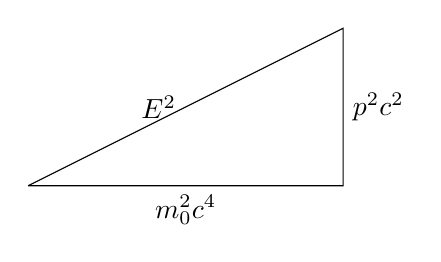
\begin{tikzpicture}
		\draw (0,0)--node[below]{$m_0^2c^4$}(4,0)--node[right]{$p^2c^2$}(4,2)--node[left]{$E^2$}(0,0);
	\end{tikzpicture}
	\caption*{能量动量三角形}
\end{figure}
\newpage
\csection{相对论中的力}
\noindent 实际上相对论在推导的时候是基于保留动量守恒定律的, 也就是修改了物理量的概念而试图保存物理定律. 那么可以根据力的定义来计算:
 $$
 \boldsymbol{F}=\dfrac{\mathrm{d}}{\mathrm{d}t}\left( \dfrac{m_0\boldsymbol{u}}{\sqrt{1-\dfrac{u^2}{c^2}}} \right) 
 $$
 展开过程是一坨大便, 略去不写:
 $$
 F_x'=F_x-\dfrac{\dfrac{u_yv}{c^2}F_y}{1-\dfrac{vu_x}{c^2}}-\dfrac{\dfrac{u_zv}{c^2}F_z}{1-\dfrac{vu_z}{c^2}}=\dfrac{F_x-\dfrac{v}{c^2}\boldsymbol{u}\cdot \boldsymbol{F}}{1-\dfrac{vu_x}{c^2}}
  $$
 $$
 F_y'=\dfrac{\dfrac{1}{\gamma}F_y}{1-\dfrac{vu_x}{c^2}}=\dfrac{F_y\sqrt{1-\dfrac{v^2}{c^2}}}{1-\dfrac{vu_x}{c^2}}
 $$
 $$
 F_z'=\dfrac{\dfrac{1}{\gamma}F_z}{1-\dfrac{vu_x}{c^2}}=\dfrac{F_y\sqrt{1-\dfrac{v^2}{c^2}}}{1-\dfrac{vu_x}{c^2}}
 $$
 
\end{document}